\chapter{Packages}
\label{ch:package}

In this chapter, all packages and their purpose are introduced.

\section{MORR}

\begin{center}
    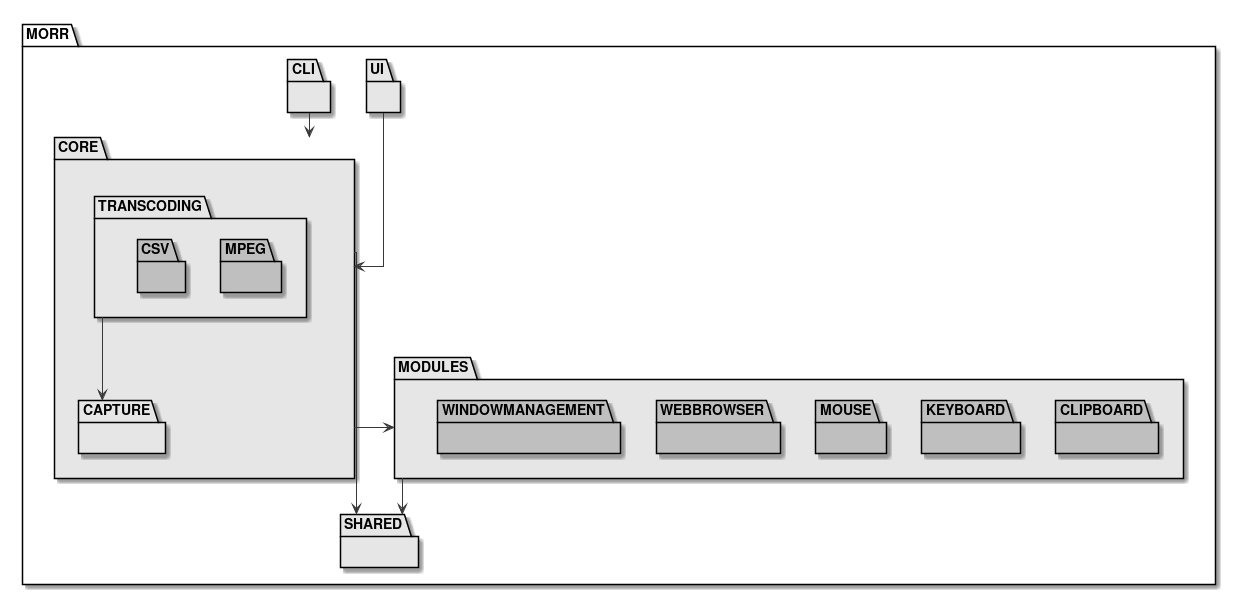
\includegraphics[width=1.0\textwidth]{resources/Packages/AllPackages.png}
\end{center}

The MORR package is the master package containing the whole application. It does not contain any classes directly as it only serves as a container for all packages required in the design.

\newpage
\section{MORR.CORE}

The \textbf{CORE} package contains the central initializing logic to be called when the program is started and coordinates state-changes while the application is running.

Contained classes:
\begin{itemize}
\item MORR 
\item Bootstrapper
\item ConfigurationManager
\item ModuleManager
\end{itemize}

\newpage
\section{MORR.CLI}

The \textbf{CLI} package contains all logic exclusively needed for the command line interface which allows for the extraction of event data from saved recordings.

Contained classes:
\begin{itemize}
\item Program
\item Executor
\item OutputFormatter
\item Options
\end{itemize}

\newpage
\section{MORR.SHARED}

The \textbf{SHARED} package provides interfaces and classes which have to be known and shared across multiple packages, such as the concept of an event or a module.

Contained interfaces:
\begin{itemize}
\item IConfiguration
\item IModule
\item ITransformingModule
\item ICollectingModule
\item IReceivingModule
\end{itemize}

Contained classes:
\begin{itemize}
\item \textit{abstract} EventQueue<T>
\item InvalidConfigurationException
\item IReadOnlyEventQueue<T>
\item \textit{abstract} Event
\item Exception
\end{itemize}

\newpage
\section{MORR.TRANSCODING}

The \textbf{TRANSCODING} package is responsible for serialization and deserialization of recorded video-, audio- and event-data. 

Contained interfaces:
\begin{itemize}
\item IVideoCapture
\item IAudioCapture
\item IDecoder
\item IEncoder
\end{itemize}

Contained classes:
\begin{itemize}
\item \textit{abstract} AudioSample
\item \textit{abstract} VideoSample
\item \textit{abstract} MetadataSample
\item DecodingException
\item EncodingException
\item CaptureException
\item MetadataDecodingException
\item AudioDecodingException
\item VideoDecodingException
\item MetadataEncodingException
\item AudioEncodingException
\item VideoEncodingException
\item VideoCaptureException
\item AudioCaptureException
\end{itemize}

\newpage
\section{MORR.MODULES}

The\textbf{MODULES} package serves as a container for all module-subpackages.

\subsection*{MORR.MODULES.WINDOWMANAGEMENT}

The \textbf{WINDOWMANAGEMENT} package is responsible for providing the classes and concepts necessary for recording the window related user-interactions.

Contained classes:
\begin{itemize}
\item WindowManagementModule
\item \textit{abstract} WindowEvent
\item WindowMovementEvent
\item WindowFocusEvent
\item WindowSateChangedEvent
\item WindowResizingEvent
\end{itemize}
\newpage
\subsection*{MORR.MODULES.KEYBOARD}

The \textbf{KEYBOARD} package is responsible for providing the classes and concepts necessary for recording the keyboard related user-inputs.

Contained classes:
\begin{itemize}
\item \textit{abstract} KeyboardEvent
\item KeyboardModule
\item KeyboardInteractEvent
\end{itemize}

\newpage
\subsection*{MORR.MODULES.WEBBROWSER}

The \textbf{WEBBROWSER} package is responsible for providing the classes and concepts necessary for recording the webbrowser related user-interactions.

Contained classes:
\begin{itemize}
\item WebBrowserModule
\item \textit{abstract} WebBrowserEvent
\item TextSelectionEvent
\item TextInputEvent
\item SwitchTabEvent
\item OpenTabEvent
\item CloseTabEvent
\item NavigationEvent
\item HoverEvent
\item FileDownloadEvent
\item ButtonClickEvent
\end{itemize}

\newpage
\subsection*{MORR.MODULES.CLIPBOARD}

The \textbf{CLIPBOARD} package is responsible for providing the classes and concepts necessary for recording the clipboard related user-interactions.

Contained classes:
\begin{itemize}
\item ClipboardModule
\item \textit{abstract} ClipboardEvent
\item ClipBoardInteractEvent
\end{itemize}

Contained enums:
\begin{itemize}
\item InteractionType
\end{itemize}

\newpage
\subsection*{MORR.MODULES.MOUSE}

The \textbf{MOUSE} package is responsible for providing the classes and concepts necessary for recording the mouse related user-inputs.

Contained classes:
\begin{itemize}
\item MouseModule
\item \textit{abstract} MouseEvent
\item MouseScrollEvent
\item MouseClickEvent
\item MouseMoveEvent
\end{itemize}

Contained enums:
\begin{itemize}
\item MouseButton
\item MouseButtonState
\end{itemize}
